\section{实数}

数学分析研究的基本对象是定义在实数集上的函数.为此,我们先简要叙述实数的有关概念.

\subsection{实数及其性质}

在中学数学课程中,我们知道实数由有理数与无理数两部分组成.\textbf{有理数} 可用分数形式 $\frac{p}{q}$ ( $p$、$q$ 为整数,$q \neq 0$) 表示,也可用有限十进制小数或无限循环十进制小数来表示; 而无限不循环十进制小数则称为\textbf{无理数}.有理数和无理数统称为\textbf{实数}.

为了之后讨论的需要,我们把有限十进制小数 (包括整数) 也统一表示为无限十进制小数.为了实现这个目的,我们作如下规定:
\begin{itemize}
    \item 对于正有限小数 $x=a_0.a_1 a_2 \cdots a_n$ 时,其中 $0 \leq a_i \leq 9$ , $i=1,2,\cdots n$ , $a_n \ne 0$ ,$a_0$ 为非负整数,记
    \[
        x = a_0.a_1 a_2 \cdots (a_n-1) 9999\cdots
    \]
    \item 对于正整数 $x=a_0$ , 记
    \[
        x = (a_0-1).9999\cdots
    \]
    \item 对于负有限小数(包括负整数) $y$ ,先将 $-y$ 表示为正无限小数,再加负号得到 $y$ 的无限小数形式
    \item 对于 0 ,记 $0=0.000 \cdots$

    于是,任何实数都可用一个确定的无限小数来表示. 如 5 表示为 4.999$\cdots$ , 3.1415 表示为 $3.14149999 \cdots$ , -2.738 表示为 $-2.7379999 \cdots$
\end{itemize}

我们已经熟知比较两个有理数大小的方法了.下面定义两个实数的大小关系.

\begin{definition}
[非负实数的大小]
 给定两个非负实数
\[
  x=a_0.a_1 a_2 \cdots a_n \cdots, \quad y=b_0.b_1 b_2 \cdots b_n \cdots
\]
其中 $a_0,b_0$ 为非负整数,$a_k,b_k(k=1,2,\cdots)$ 为整数,$0\le a_k \le 9,0\le b_k \le 9$.

\textbullet 若有 $a_k = b_k(k=0,1,2,\cdots)$ ,则称 $x$ 与 $y$ 相等 ,记为 $x=y$.
    
\textbullet 若 $a_0>b_0$ 或存在非负整数 $l$ ,使得 $a_k = b_k(k=0,1,2,\cdots,l)$ 但 $a_{l+1}>b_{l+1}$ ,则称 $x$ 大于 $y$ 或 $y$ 小于 $x$ ,记为 $x>y$ 或 $y<x$.

\qquad 对于负实数 $x,y$ ,如果按照上面的定义,分别有$-x=-y$ 与 $-x>-y$ ,则分别称 $x=y$ 与 $x<y$ (或 $y>x$).

\qquad 另外,规定任何非负实数大于任何负实数.    
\end{definition}

下面给出一个通过有限小数来比较两个实数大小的等价条件.为此,先给出如下定义.

\begin{definition}[实数的近似]
    设 $x=a_0.a_1 a_2 \cdots a_n \cdots$ 为非负实数.

    \textbullet 称有理数 $x_n=a_0.a_1 a_2 \cdots a_n$ 为实数 $x$ 的 \textbf{n位不足近似}.

    \textbullet 称有理数 $\bar x_n=x_n + \frac{1}{10^n}$ 为 $x$ 的 \textbf{n位过剩近似}.

    对于负实数 $x=-a_0.a_1 a_2 \cdots a_n \cdots$ , 其 n 位不足近似和 n 位过剩近似分别规定为
    \[
      x_n = -a_0.a_1 a_2 \cdots a_n - \frac{1}{10^n} \qquad \bar x_n = x_n +\frac{1}{10^n}
    \]
\end{definition}

\begin{annotation}
    不难看出, 实数 $x$ 的不足近似 $x_n$ 当 $n$ 增大时不减,即 $x_0 \le x_1 \le x_2 \le \cdots$; 而过剩近似 $\bar x_n $ 当 $n$ 增大时不增,即 $\bar x_0 \ge \bar x_1 \ge  \bar x_2 \ge \cdots$
\end{annotation}

我们有以下的命题.

\begin{proposition}[近似等价比大小]\label{pro:about}
    设 $x=a_0.a_1a_2\cdots$ 与 $y=b_0.b_1b_2\cdots$ 为两个实数,则
    \[
    x>y \iff \exists n\in N , \mbox{使得} x_n > \bar y_n
    \]
    其中,$x_n$ 表示 $x$ 的 n位不足近似, $\bar y_n$ 表示 y 的n位过剩近似.
\end{proposition}

关于这个命题的证明,以及实数四则运算的定义,可参阅本书附录。

\begin{example}[两个实数之间必定存在有理数]\label{ex:inside}
    设 $x$,$y$为实数,$x<y$.证明: 存在有理数 $r$,满足 $x<r<y$.
\end{example}

\begin{proof}
    $x<y$,由 \proref{pro:about} 得,存在非负整数 $n$ ,使得$\bar x_n < y_n$.

    令 $r=\frac{1}{2}(\bar x_n + y_n)$ ,则 $r$ 为有理数,且有
    \[
    x \le \bar x_n < r < y_n \le y
    \]
\end{proof}

为了方便起见,通常将全体实数构成的集合记为 $\mathbb{R}$ ,即 $\mathbb{R}=\{x\mid x\mbox{为实数}\}$.

实数有如下一些主要性质:

\begin{enumerate}
    \item 实数集 $\mathbb{R}$ 对加、减、乘、除(除数不为 0)四则运算是封闭的,即任意两个实数的和、差、积、商(除数不为 0)仍然是实数.
    \item 实数集是有序的,即任意两实数 $a,b$ 必然满足下述三个关系之一:$a<b,a=b,a>b$.
    \item 实数的大小关系具有传递性,即若 $a>b,b>c$ ,则有 $a>c$.
    \item 实数具有阿基米德(Archimedes)性,即对任何 $a,b\in \mathbb{R}$ ,若 $b>a>0$ ,则存在正整数 $n$,使得 $na>b$.
    \item 实数集 $\mathbb{R}$ 具有稠密性,即任何两个不相等的实数之间必有另一个实数,且既有有理数(见\exref{ex:inside}),也有无理数.
    \item 如果在一条直线上(通常画成水平直线)确定一点 $O$ 作为原点,指定一个方向为正向(通常把指向右方的方向规定为正向),并规定一个单位长度,则称此直线为 \textbf{数轴}.可以说明:任一实数都对应数轴上唯一的一点;反之,数轴上的每一点也都唯一地代表着一个实数.于是,实数集 $\mathbb{R}$ 与数轴上的点有着一一对应关系.在本书以后的叙述中,常把“实数 $a$” 与“数轴上的点$a$” 这两种说法看做具有相同的含义.
\end{enumerate}

\begin{example}
    设 $a,b\in \mathbb{R}$.证明:若对任何正数 $\varepsilon$ ,有 $a<b+\varepsilon$ ,则 $a \le b$.
\end{example}

\begin{proof}
    用反证法.假设结论不成立,则根据实数集的有序性,必有 $a>b$ .令 $\varepsilon=a-b$ ,则 $\varepsilon$ 为正数,但有 $a=b+\varepsilon$ ,这与题设 $a<b+\varepsilon$ 产生矛盾.因此必有 $a\le b$.
\end{proof}

\subsection{绝对值与不等式}

实数 $a$ 的\textbf{绝对值} 定义为
\[
 \mid a \mid= 
\begin{cases}
    a,&  a\ge 0 \\
    -a,& a<0 \\
\end{cases}
\]
从数轴上看,数 $a$ 的绝对值 $\mid a \mid$ 就是点 $a$ 到原点的距离.

实数的绝对值有如下一些性质:
\begin{enumerate}
    \item $\abs{a} = \abs{-a} \ge 0$ , 当且仅当 $a=0$ 时,有 $\abs{a}=0$.
    \item $-\abs{a} \le a \le \abs{a}$.
    \item $\abs{a} < h \iff -h < a < h$ \qquad $\abs{a} \le h \iff -h \le a \le h$  (h>0).
    \item 对任何 $a,b \in \mathbb{R}$ ,都有如下的\textbf{三角不等式}:
    \[
    \abs{a} - \abs{b} \le \abs{a \pm b} \le \abs{a} + \abs{b}
    \]
    \item $\abs{ab} = \abs{a}\abs{b}$
    \item $ \abs{\frac{a}{b}}= \frac{\abs{a}}{\abs{b}}(b\ne 0)$
\end{enumerate}

下面只证明性质4,其余性质由读者自行证明.

\begin{proof}
    由性质2有 \qquad $-\abs{a} \le a \le \abs{a},-\abs{b} \le b \le \abs{b}$

    两式相加得 \qquad $- (\abs{a}+\abs{b}) \le a+b \le \abs{a}+\abs{b}$

    根据性质3,上式等价于
    \begin{equation}
        \abs{a+b} \le \abs{a}+\abs{b}
    \end{equation}
    
    将 式(1) 中 $b$ 换成 $-b$, 即得 $\abs{a-b} \le \abs{a}+\abs{-b}=\abs{a}+\abs{b}$ ,这就证明了性质4不等式的右半部分.

    又由 $\abs{a} = \abs{a-b+b}$ ,根据式 (1.1) 得 $ \abs{a} \le \abs{a-b}+\abs{b}$,从而有
    \begin{equation}
        \abs{a} - \abs{b} \le \abs{a-b}
    \end{equation}

    将 式(2) 中的 $b$ 换成 $-b$ ,即得 $\abs{a} - \abs{b} \le \abs{a + b}$.左半部分得证.
\end{proof}

\homework

\begin{practice}
    设 $a$ 为有理数, $x$ 为无理数.证明:
    
   (1) $a+x$ 是无理数 \quad (2) 当 $a\ne 0$ 时, $ax$ 是无理数.
\end{practice}

\begin{proof}
    (1) 用反证法.假设 $a+x$ 是有理数,则存在整数$q_1,p_1\ne 0$ 使得 $a+x = \frac{q_1}{p_1}$. 又 $a$ 为有理数,则 存在整数$q_2,p_2\ne 0$ 使得 $a= \frac{q_2}{p_2}$.
    则 $x=(a+x)-a=\frac{q_1}{p_1}-\frac{q_2}{p_2}=\frac{q_1p_2-q_2p_1}{p_1p_2}$.其中, $q_1p_2-q_2p_1$,$p_1p_2$均为整数,且$p_1p_2\ne 0$,则 $x$ 也为有理数.这与题设 $x$ 为无理数相矛盾.故 $a+x$ 必为无理数.

    (2) 与 (1) 思路类似.假设 $ax$ 是有理数,有 $ax=\frac{q_1}{p_1},a=\frac{q_2}{p_2}$,其中 $p_1,p_2,q_2$ 均不为0. 则 $x=\frac{ax}{a}=\frac{q_1p_2}{p_1q_2}$也为有理数.与题设矛盾.
\end{proof}

\begin{practice}
    试在数轴上表示出下列不等式的解:
    
    (1) $x(x^2-1)>0$ \quad (2) $\abs{x-1} < \abs{x-3}$ \quad (3)$\sqrt{x-1}-\sqrt{2x-1} \ge \sqrt{3x-2}$
\end{practice}

\begin{solve}
    (1) 因式分解得 $x(x+1)(x-1)>0 \implies -1<x<0 \mbox{或} x>1$
    
    {\vspace{0.1cm}\hfill\begin{tikzpicture}
        \nlAxisX{-2}{2}
        \nlnumnum{-1}{o}{0}{o}
        \nlnuminf{1}{o}
    \end{tikzpicture}\hfill}

    (2)两边平方得 $(x-1)^2<(x-3)^2 \implies 4x<8 \implies x<2$.

    {\vspace{0.1cm}\hfill\begin{tikzpicture}
        \nlAxisX{-1}{3}
        \nlinfnum{2}{o}
    \end{tikzpicture}\hfill}

    (3) 首先,根据平方根的非负性,有 $x-1\ge 0,2x-1\ge 0,3x-2\ge 0,x-1\ge 2x-1$

    整理得相互矛盾的不等式:$x\ge 1,x\le 0$. 故不等式无解.
\end{solve}

\begin{practice}
    设 $a,b\in \R$.证明:若对任何正数 $\varepsilon$ ,都有 $\abs{a-b}<\varepsilon$ ,则 $a=b$.
\end{practice}

\begin{proof}
    用反证法.假设 $a\ne b$ ,则 $\abs{a-b}>0$. 取 $\varepsilon = \abs{a-b}$ ,则 $\abs{a-b}=\varepsilon$. 这与题设$\abs{a-b}<\varepsilon$相矛盾.故必有 $a=b$.
\end{proof}

\begin{practice}
    设 $x\ne 0$ ,证明 $\abs{x+\frac{1}{x}}\ge 2$ ,并说明其中等号何时成立.
\end{practice}

\begin{proof}
    易知 $(x-\frac{1}{x})^2\ge 0 \iff x^2-2+\frac{1}{x^2}\ge 0 \iff x^2+2+\frac{1}{x^2} \ge 4 \iff (x+\frac{1}{x})^2\ge 4 \iff (\abs{x+\frac{1}{x}}) \ge 2^2 \iff \abs{x+\frac{1}{x}}\ge 2$. 并且, $\abs{x+\frac{1}{x}}= 2 \iff (x-\frac{1}{x})^2= 0\iff x=\frac{1}{x} \iff x^2=1 \iff \abs{x}=1$. 即 $\abs{x}=1$ 时等号成立.
\end{proof}

\begin{practice}
    证明:对任何 $x\in \R$ ,有

    (1)$\abs{x-1} + \abs{x-2} \ge 1$ \quad (2)$\abs{x-1} + \abs{x-2} + \abs{x-3} \ge 2$
\end{practice}

\begin{proof}
    (1) 由三角不等式得 $\abs{x-1} + \abs{x-2} \ge \abs{(x-1)-(x-2)}=1$.当且仅当 $x-1\ge 0$ 且 $x-2\le 0$,即 $x\in [1,2]$ 时等号成立.

    (2) $\abs{x-1} + \abs{x-2} + \abs{x-3} \ge \abs{x-1} + \abs{x-3} \ge \abs{(x-1)-(x-3)}=2$. 当且仅当 $x = 2$ 时等号成立.
\end{proof}

\begin{practice}
    设 $a,b,c \in \R^+$ ($\R^+$ 表示全体正实数的集合).证明:
    $$\abs{\sqrt{a^2+b^2}-\sqrt{a^2+c^2}} \le \abs{b-c}.$$

    你能说明此不等式的几何意义吗?
\end{practice}

\begin{proof}
欲证 $\abs{\sqrt{a^2+b^2}-\sqrt{a^2+c^2}} \le \abs{b-c}$

只需证 $(\abs{\sqrt{a^2+b^2}-\sqrt{a^2+c^2}})^2 \le (\abs{b-c})^2$

$\iff a^2 + b^2 + 2\sqrt{(a^2+b^2)(a^2+c^2)} + b^2 + c^2 \le b^2 + 2bc + c^2\iff a^2 + bc \le \sqrt{(a^2+b^2)(a^2+c^2)}$

$\iff a^4 + 2a^2bc + b^2c^2 \le a^4 + a^2c^2 + a^2b^2 +b^2c^2$

$\iff 2a^2bc \le a^2(b^2+c^2)$

由于 $a^2\ge 0$ 且 $b^2+c^2\ge 2bc$ ,故原命题得证.

几何意义:给出平面上两点 $A(a,b),B(a,c)$,则 $A,B$ 到原点 $O$ 的距离分别为 $\sqrt{a^2+b^2},\\ \sqrt{a^2+c^2}$ , $A,B$ 两点的距离为 $\abs{b-c}$ .故原不等式等价于 $\abs{OA-OB}\le \abs{AB}$ ,即两边之差小于第三边.如下图所示.

{\vspace{0.1cm}\hfill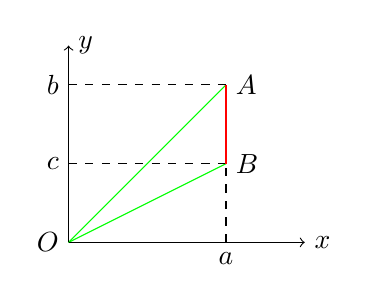
\begin{tikzpicture}
    \node at (0,0) [left] {$O$};
    \node at (0,1) [left] {$c$};
    \node at (0,2) [left] {$b$};
    \node at (2,0) [below] {$a$};
    \node at (2,1) [right] {$B$};
    \node at (2,2) [right] {$A$};
    \draw[-,color=green] (0,0)--(2,1) ;
    \draw[-,color=green] (0,0)--(2,2) ;
    \draw[->] (0,0)--(3,0) node[right] {$x$};
    \draw[->] (0,0)--(0,2.5) node[right] {$y$};
    \draw[-,dashed] (0,2)--(2,2);
    \draw[-,dashed] (0,1)--(2,1);
    \draw[-,dashed] (2,0)--(2,2);
    \draw[-,color=red] (2,1)--(2,2);
\end{tikzpicture}\hfill}

\quad
\end{proof}

\begin{practice}
    设 $x>0,b>0,a\ne b$.证明 $\frac{a+x}{b+x}$ 介于 $1$ 与 $\frac{a}{b}$ 之间.
\end{practice}

\begin{proof}
\begin{align*}
    &(\frac{a+x}{b+x}-1)(\frac{a+x}{b+x}-\frac{a}{b}) \\
    &= (\frac{a+x-b-x}{b+x})(\frac{ab+bx-ab-ax}{b(b+x)}) \\
    & =\frac{-x(a-b)^2}{b(b+x)^2}
\end{align*}

由于 $x>0,b>0,a\ne b$ ,上式 $<0$. 故$\frac{a+x}{b+x}$ 介于 $1$ 与 $\frac{a}{b}$ 之间.
\end{proof}

\begin{practice}
    设 $p$ 为正整数.证明: 若 $p$ 不是完全平方数,则 $\sqrt{p}$ 是无理数.
\end{practice}

\begin{proof}
    用反证法.假设 $\sqrt{p}$ 是有理数,则存在互质的正整数 $m,n$ 使得 $\sqrt{p} = \frac{n}{m} \iff p=\frac{n^2}{m^2}$. 可得 $n^2 = p m^2$ ,于是 $p$ 是 $n$ 的因数. 设 $n=pk$ ,则 $k$ 与 $m$互质,且$p^2k^2 = pm^2 \iff m^2 = pk^2$. 可得 $p$ 也是 $m$ 的因数. $m,n$ 有公因数 $p$ ,这与 $m,n$ 互质相矛盾. 故$\sqrt{p}$ 是无理数.
\end{proof}

\begin{practice}
    设 $a,b$ 为给定实数.试用不等式符号(不用绝对值符号)表示下列不等式的解:

    (1) $\abs{x-a} < \abs{x-b}$ \quad (2) $\abs{x-a} < x-b$ \quad (3) $\abs{x^2-a}<b$
\end{practice}

\begin{solve}
    (1) \begin{align*}
    &\abs{x-a} < \abs{x-b} \\
    & \iff (x-a)^2 < (x-b)^2  \iff 2x(a-b) > a^2 + b^2\\
    & \iff \begin{cases}
        \mbox{无解} & a=b \\ 
        x > \frac{a+b}{2} & a>b \\ 
        x < \frac{a+b}{2} & a<b \\ 
    \end{cases}
\end{align*}

(2) 解集必然是 $\{x \mid x>b\}$ 的子集. 结合 (1) 可得
$$\begin{cases}
        \mbox{无解} & a\le b \\ 
        x > \frac{a+b}{2} & a>b \\ 
    \end{cases}$$

(3) <1>当 $b\le 0$ 时, 不等式无解.

\hspace{1.4em} <2>当 $b>0$ 时,不等式等价于 $a-b < x^2 < a+b$.

\qquad \qquad [1]当 $a+b\le 0$ 时,不等式无解. 

\qquad \qquad[2] 当  $a+b> 0$ 时,

\qquad \qquad \qquad 1)若 $a<b$ ,不等式的解为 $-\sqrt{a+b} < x < \sqrt{a+b}$ .

\qquad \qquad \qquad 2)若 $a>b$ ,不等式的解为 $\sqrt{a-b} < x < \sqrt{a+b}$ 或  $-\sqrt{a+b} < x < -\sqrt{a-b}$.
\end{solve}

\newsection